Problem harmonogramowania

Obecnie podstawą zarządzania wszelkiego rodzaju projektami jest proces harmonogramowania. Pod tym terminem kryje się nic innego jak planowanie najbardziej optymalnej sekwencji operacji mające na celu zminimalizowanie czasu ich wykonania. Oczywistą korzyścią jest najlepsze wykorzystaniu czasu oraz możliwość dokładnego obliczenia terminu wykonania całego przedsięwzięcia, lub jego części. Harmonogram ułatwia również śledzenie zależności między pojedynczymi procesami oraz pozwala na wczesne wykrywanie zagrożeń realizacji. Do graficznego przedstawienia wspomnianego procesu, najczęściej używany jest wykres Gantta. 

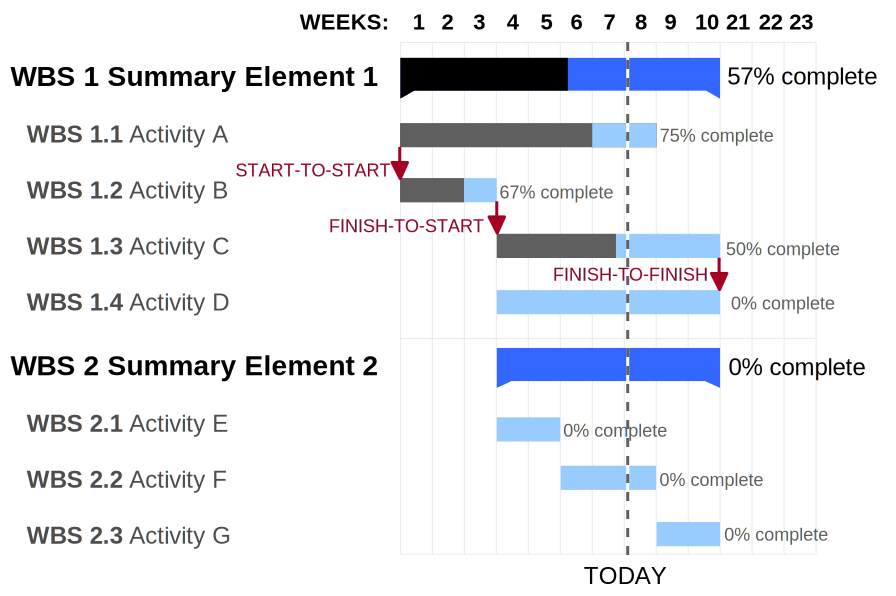
\includegraphics{Grafika/wykres-gantt.svg}

Do wyznaczenia optymalnej kolejności opracowano wiele algorytmów, zarówno dokładnych jak i przybliżonych, z których najważniejsze to:

* Johnsona
* Campbella-Dudka-Smitha
* Browna-Łomnickiego

Wspomniane algorytmy zostaną omówione na przykładzie obróbki m detali na n maszynach. Dodatkowo, poniżej zostały sprecyzowane założenia, które muszą być spełnione:

* każdy detal jest obrabiany dokładnie raz na każdej maszynie
* czasy obróbki każdego detalu na każdej maszynie są znane
* nie można rozpocząć procesu obróbki kolejnego detalu zanim nie zostanie zakończony poprzedni
* kolejność procesu obróbki jest identyczna dla wszystkich detali z danej partii oraz każdej maszyny
 
Algorytm Johnsona

Wspomniany algorytm możliwy jest do użycia tylko w wypadku kiedy mamy 2 lub 3 maszyny do obróbki detali oraz poniższą macierz z czasami obróbki 

\begin{pmatrix} t_{1,1} & t_{1,2} & \cdots & t_{1,j} \\ t_{2,1} & t_{2,2} & \cdots & t_{2,j} \end{pmatrix}

1) Znajdujemy min t_{i,j}
2) Jeżeli min t_{i,j} = t_{1,k} to optymalna kolejność musi się rozpocząć od obróbki detalu o indeksie k natomiast jeżeli min t_{i,j} = t_{2,s} to musi zakończyć się detalem o indeksie s
3) Wykreślamy z powyższej macierzy czasów, komunę i ze znalezionym w drugim kroku minimum oraz wracamy do pierwszego kroku zakładając że znaleziony min t_{i,j} ustawia się w pierwszym wolnym miejscu, odpowiednio od końca lub początku.
